\section{Diario della riunione}
\begin{itemize}
  \item Discusso e normato l'utilizzo di base di Trello come principale kanban per la gestione del progetto; le regole principali sono:
  \begin{itemize}
    \item Board principale divisa nelle seguenti colonne formanti una pipeline: \textit{Backlog, Todo, Doing, Verify, Done};
    \item Ogni task nelle fasi di \textit{Doing, Verify, Done} è assegnata a uno o più membri (assenza di "task orfane");
    \item Ogni task in \textit{Todo, Verify} può essere autonomamente presa in carico da un qualsiasi membro del gruppo (coerentemente a: stato della task, ruolo, accordi preesistenti);
    \item Ogni task che entra nella pipeline ad esclusione del \textit{Backlog} non può essere eliminata ma solo avanzare nella pipeline (tracciabilità delle tasks).
  \end{itemize}
  \item Assegnati i documenti da redigere e da verificare a ciascun membro del gruppo, in modo da riuscire a coprire al meglio tutti i ruoli di progetto;
  
\begin{center}
  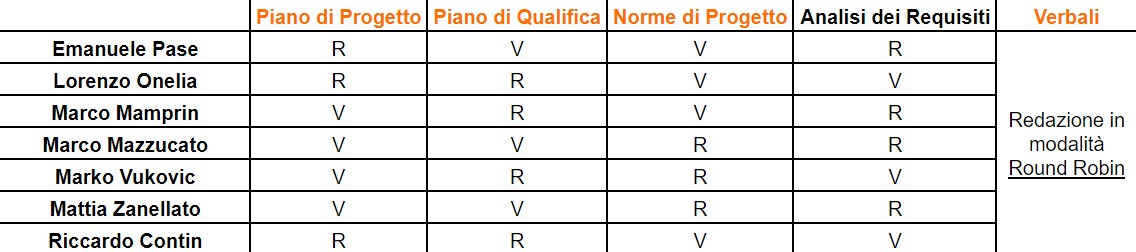
\includegraphics[width=0.8\textwidth]{documenti}
\end{center}
  
  \item Normato e automatizzato mediante Google Sheets un elementare sistema di consuntivo delle ore produttive individuali settimanali e totali;
  \item Discusso e normato l'utilizzo di base di Google Calendar come strumento per tracciare scadenze (interne ed esterne) ed eventi;
  \item Stabilito metodo di turnazione round robin per la redazione di verbali;
  \item Stabilita deadline interna per la RTB al \textit{14/01/2022};
  \item Pianificato riallineamento del gruppo sulle competenze di base degli strumenti: \textit{Git, GitHub, LaTeX}.
\end{itemize}